\chapter{Safety}
\label{chapter:safety}


In this manual, safety instructions and observations are highlighted by boxes.
\section{Feedback}

If you encounter a dangerous situation that is specific to {\projectname} and is not covered by the rules below or if you have comments or suggestions on the existing rules, please inform the leaders of {\projectname}
\ifcoatli
(Alan Watson and Salvador Cuevas)
\fi
\ifddoti 
(Alan Watson and William Lee) 
\fi
and the Secretario Técnico of the OAN.

\section{Priorities}

\safety{
The safety priorities at {\projectname}, from highest to lowest, are:
\begin{enumerate}
\item Avoiding injury and death to personnel.
\item Avoiding damage or loss of equipment.
\item Observing and data preservation.
\end{enumerate}
}

\section{Personnel Safety}

The {\projectname} installation is potentially one of the most dangerous installations at the OAN/SPM. Personnel safety is more important than equipment safety or observations. The following  rules are designed to maintain personnel safety and must be followed at all times.

\safety{You must not work alone on the open platform or on the balconies.} 

At least one other person must be present either on the platform or at ground level.

\safety{You may work alone on the closed platform. However, someone else must be present when you ascend or descend.}

You should have someone to close the enclosure manually after you have entered and open it manually for you to leave. Remember that you must have a radio on hand.

\safety{You must use a safety harness, line, and helmet whenever you are on the  platform or balconies or to ascend the tower. When you are working on the balcony or another position from which you might fall, attach your line to one of the eyes, to the balcony rail, or to something equivalently strong. In cold weather, we strongly recommend using gloves.} 

The main platform is about 5 meters above the walkways. A fall from this height can easily kill.

Safety harnesses, lines, and helmets are stored in the shed.

The line can be attached to various points: the eyes in the platform floor and balconies installed specifically for this purpose, the balcony safety rails, and other parts of the platform or tower structure.

The helmet will protect you from collisions with the telescopes, if you fall, and from falling objects.

\safety{You must use a safety helmet if you are working under the platform or balconies.}

The main platform is about 5 meters above the walkways. An impact from an object falling from this height can easily kill.

Safety helmets are stored on the shed.

\safety{Transport equipment and tools to and from the platform using the appropriate equipment provided: ropes, locking carabiners, locking hooks, straps, a tool carrier, and an equipment bag.}

This equipment, shown in Figure~\ref{figure:safety-transport}, is stored in the project cabinet in the ground-floor of the 84-cm telescope. Using this equipment in an appropriate manner will significantly reduce the risk of something falling. When you use the rope, you can fasten the upper end to one of the eyes in the platform using a locking carabiners. When lifting heavy equipment to the platform, consider using the locking hook.

\begin{figure}
\begin{center}
\resizebox{\linewidth}{!}{
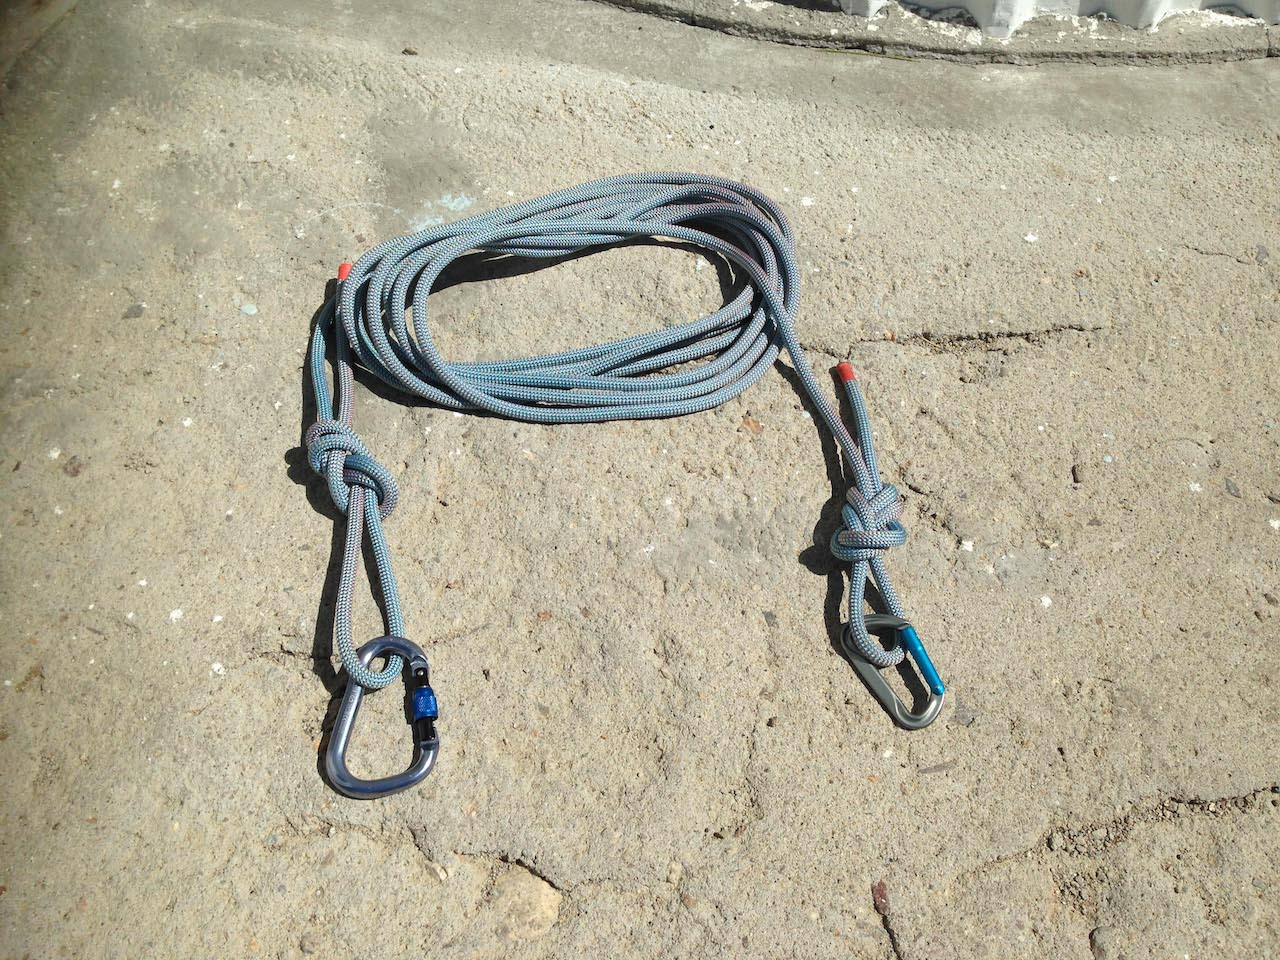
\includegraphics[width=0.50\linewidth]{figures/safety-rope}
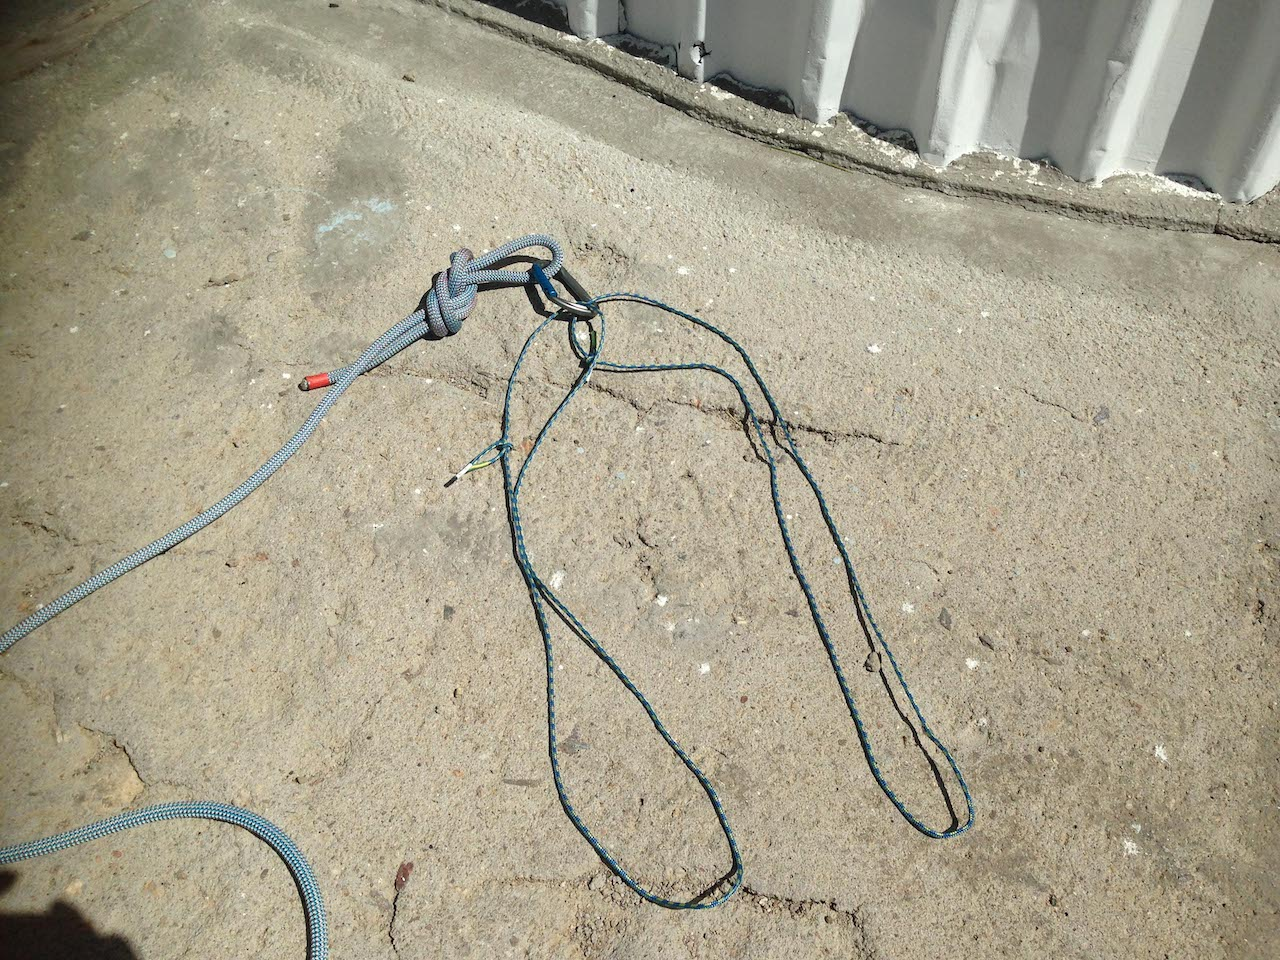
\includegraphics[width=0.50\linewidth]{figures/safety-straps.jpg}
}
\resizebox{\linewidth}{!}{
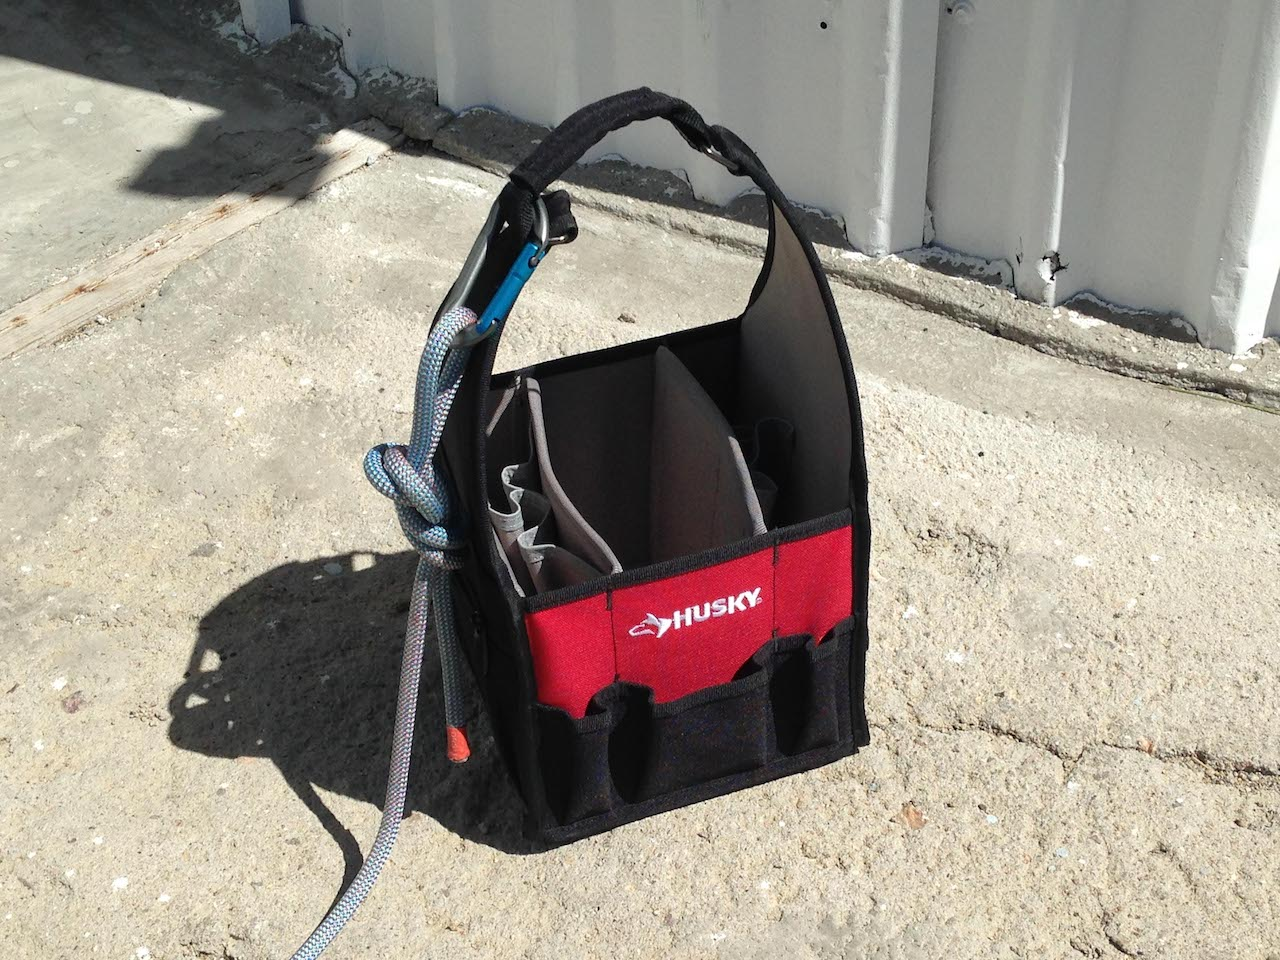
\includegraphics[width=0.50\linewidth]{figures/safety-tools.jpg}
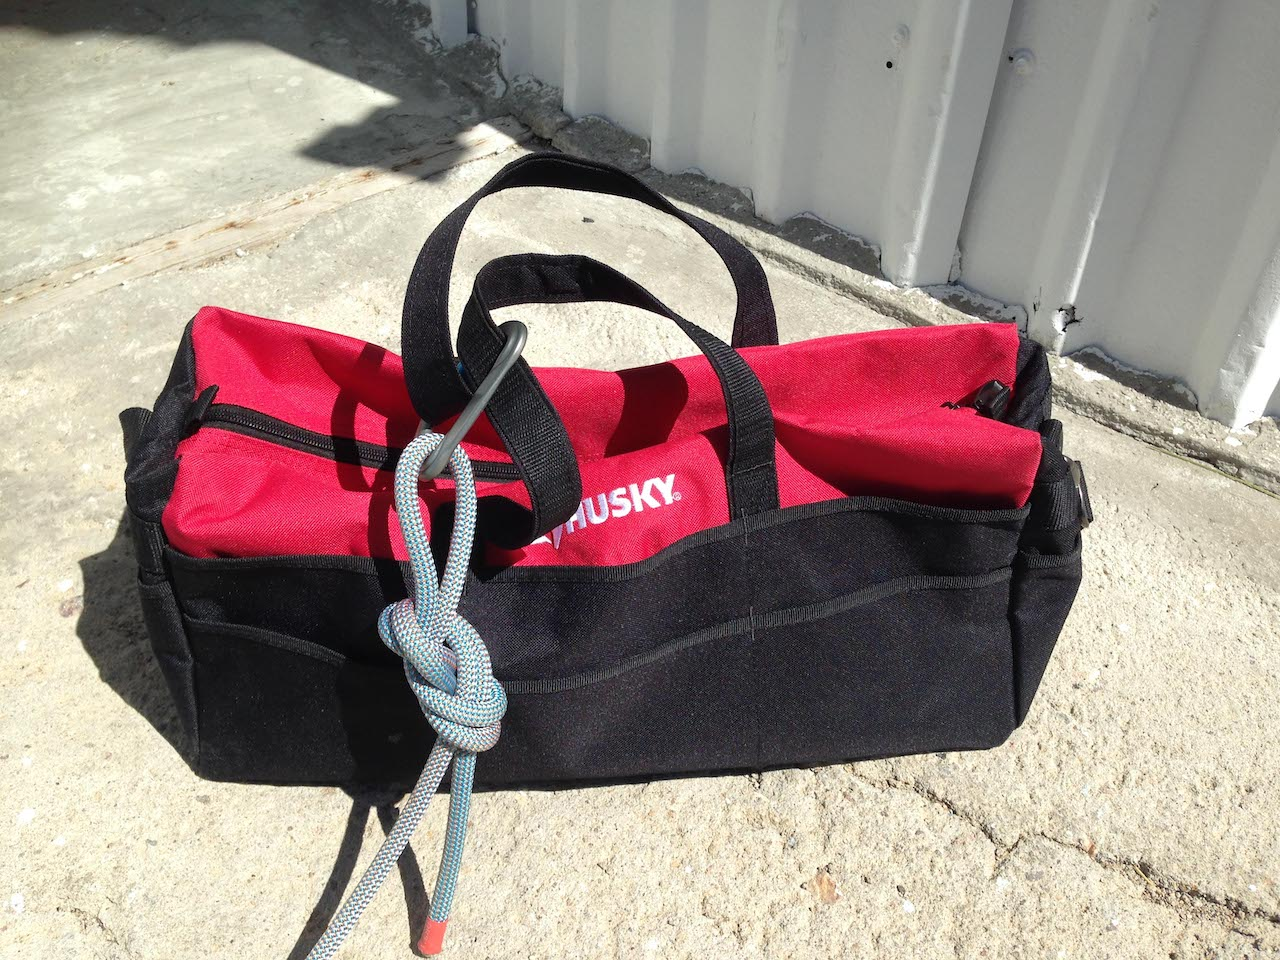
\includegraphics[width=0.50\linewidth]{figures/safety-bag.jpg}
}
\end{center}
\caption{Equipment to safely transport equipment to and from the platform: ropes, locking carabiners, straps, a tool carrier, and an equipment bag.}
\label{figure:safety-transport}
\end{figure}

\safety{Return equipment and tools to their usual storage location when you have finished using them.}

This ensures that equipment can be found when it is next needed. This is especially important for safety equipment.

\safety{If you wish to ascend to the platform or balconies, you must put the enclosure in local mode.}

In remote mode the enclosure can close without warning.

\safety{You may only be on the platform or balconies if it is strictly necessary.}

The platform and balconies are not a vantage points. You must only be on them to work on equipment.

\safety{You may only be on the platform or balconies at night if you need to close the enclosure manually or are commissioning, testing, or tuning equipment on the sky.}

If there is a failure at night, you must not ascend to the platform to fix it. Instead, you must abandon the night’s observations and attempt to close the enclosure from the shed. You may only ascend to the platform at night if you need to close the enclosure manually.

\safety{You may only be on the platform or balconies in poor conditions if you need to close the enclosure manually.}

Poor conditions include high wind, snow, and rain. 

You must not perform maintenance in poor conditions.

You may only climb the platform in poor conditions if you need to close the enclosure manually.

\safety{Do not walk on the elevated areas at the ends of the platform.}

These areas are not load-bearing. If you walk on them, it is likely that they will collapse and you will fall.

\safety{If you need to summon help and do not have a portable radio, you can use the static emergency radio located between the 84-cm building and DDOTI.} 

\safety{You must physically disconnect mains power before working on an electronics box.}

Note that box C has two mains connectors, one for regulated power and one for unregulated power. The other boxes have only one mains connector, for regulated power.

Using the switch is not enough; it is present to allow the equipment to be rebooted. Besides, the unregulated power to box C is not switched.

\safety{Be extremely careful when working inside the enclosure, covers, and secondary cabinets as they use 220 VAC.}


\section{Equipment Safety}

\safety{Only open the enclosure explicitly when conditions are benign.
Conditions are not benign if:
\begin{enumerate}
\item It is raining or snowing.
\item The humidity is 85\% or higher and rising or previously reached 90\% and has not yet fallen below 80\%.
\item The wind average speed has been {\windlimit} km/h or greater at any moment in the previous 30 minutes.  
\item There are other circumstance which, in the judgement of observatory technical staff, dictate that it is not safe to open.
\end{enumerate}
}

These rules are implemented in the {\projectname} weather server. If you check the {\projectname} web interface (see \S\ref{chapter:interface}), there is a summary line for the weather that says “may be open”, conditions are benign and you may open. If it does not, conditions are not benign and you must not open.

Note that the rules for opening the other telescopes specify a wind limit of 45 km/h. The limit for {\projectname} is currently lower until we have greater confidence in its reliability and performance in high winds.

\safety{Before opening the enclosure, check on the webcams in the interface (see \S\ref{chapter:interface}) that the telescope is not pointed to towards the sun.}

\ifcoatli
In the home position, the telescope is pointed to the north pole with the telescope above the mount.
\fi
\ifddoti
In the home position, the telescope is pointed to the north pole with the telescopes to the east and west of the mount.
\fi


\safety{The enclosure controller (see \S\ref{chapter:enclosure}) should normally be switched on at all times in order to keep the electromagnetic lock activated.}

If the lock is not activated, the wind can open the roof a few centimeters and allow the ingress of rain or snow.

\safety{In case of fire, there is an extinguisher in the shed.}

If you do fight a fire, remember that personnel safety is more important than equipment safety.

